\documentclass[12pt,english,a4paper]{article}
%\usepackage{babel}
\usepackage[utf8]{inputenc}
\usepackage{amsmath}
\usepackage{amssymb}
%\usepackage{calc}
\usepackage{graphicx}
\usepackage{float}
\usepackage{color}
\usepackage{physics}
\usepackage{listings}
\usepackage{subcaption}
\usepackage{siunitx}
\usepackage{todonotes}
\usepackage[version=4]{mhchem}
\usepackage{hyperref}
\usepackage{multirow}
\usepackage{tikz}
\usetikzlibrary{shapes,arrows}
\usepackage{mhchem}
\usepackage{pdfpages}
\usepackage{verbatim}
\usepackage{tabularx}
\usepackage{tabulary}
\usepackage{subcaption}
\usepackage{fancyhdr}



%To remove the shitty linespace in new sections DOES NOT WORK
\setlength{\parindent}{0cm}
\setlength{\parskip}{1em}
%to here



% Define block styles
\tikzstyle{decision} = [diamond, draw, fill=blue!20, 
text width=4.5em, text badly centered, node distance=3cm, inner sep=0pt]
\tikzstyle{block} = [rectangle, draw, fill=blue!20, 
text width=5em, text centered, rounded corners, minimum height=4em]
\tikzstyle{line} = [draw, -latex']
\tikzstyle{cloud} = [draw, ellipse,fill=red!20, node distance=3cm,
minimum height=2em]
%to here



%to cheat margins on paper
%\usepackage[margin=1.3cm, includeheadfoot]{geometry}




%kilder anders style
%\usepackage[backend=biber,citestyle=numeric-comp,bibstyle=numeric,sorting=none]{biblatex}
\usepackage[backend=bibtex,
style=numeric,
bibencoding=ascii
%style=alphabetic
%style=reading
]{biblatex}











\renewcommand{\exp}[1]{\mathrm{e}^{#1}}


%for text boxes
\usepackage{fancybox}
\usepackage{framed}
\usepackage{color}
\definecolor{shadecolor}{rgb}{1,0.8,0.3}
%to here

%defining QED box
\newcommand*{\QED}{\hfill\ensuremath{\square}}%
%


\definecolor{codegreen}{rgb}{0,0.6,0}
\definecolor{codegray}{rgb}{0.5,0.5,0.5}
\definecolor{codepurple}{rgb}{0.58,0,0.82}
\definecolor{backcolour}{rgb}{0.95,0.95,0.92}
\lstset{showstringspaces=false,
	basicstyle=\ttfamily,
	keywordstyle=\color{codegreen},
	commentstyle=\color{magenta},
	numberstyle=\tiny\color{codegray},
	stringstyle=\color{codepurple},
	breaklines=true,
	literate={0}{{\textcolor{blue}{0}}}{1}%
	{1}{{\textcolor{blue}{1}}}{1}%
	{2}{{\textcolor{blue}{2}}}{1}%
	{3}{{\textcolor{blue}{3}}}{1}%
	{4}{{\textcolor{blue}{4}}}{1}%
	{5}{{\textcolor{blue}{5}}}{1}%
	{6}{{\textcolor{blue}{6}}}{1}%
	{7}{{\textcolor{blue}{7}}}{1}%
	{8}{{\textcolor{blue}{8}}}{1}%
	{9}{{\textcolor{blue}{9}}}{1}%
	{.0}{{\textcolor{blue}{.0}}}{2}% Following is to ensure that only periods
	{.1}{{\textcolor{blue}{.1}}}{2}% followed by a digit are changed.
	{.2}{{\textcolor{blue}{.2}}}{2}%
	{.3}{{\textcolor{blue}{.3}}}{2}%
	{.4}{{\textcolor{blue}{.4}}}{2}%
	{.5}{{\textcolor{blue}{.5}}}{2}%
	{.6}{{\textcolor{blue}{.6}}}{2}%
	{.7}{{\textcolor{blue}{.7}}}{2}%
	{.8}{{\textcolor{blue}{.8}}}{2}%
	{.9}{{\textcolor{blue}{.9}}}{2}%
}




%erik COMPFYS
\newcommand{\gray}[1]{\textcolor{gray}{#1}}
\newcommand{\spin}[1]{\ifthenelse{#1 = 1}{\color{black}{\uparrow} }{\color{black}{\downarrow}} }
\newcommand{\tilstand}[4]{
	\(\displaystyle
	\begin{matrix}
	
	\spin{#1}  & \spin{#2}\\
	\spin{#3} & \spin{#4}
	
	\end{matrix}
	\)
}%hit








\addbibresource{kilder.bib}
\begin{document}
	\author{Thomas Aarflot Storaas\\
		\textbf{Github: \href{https://github.com/thoast/Project_4}{Projectfolder}}}
	\title{Project 4\\ a study of magnetic systems and phase transitions}
	\maketitle

\tableofcontents

\abstract{The two dimensional Ising model was studied using Monte Carlo simulations with the Metropolis algorithm. As a reference both analytical and numerical approaches to a $2\times2$ lattice. There was a good correspondence between the numerical and analytical values. Convergence of the system was reached when an approximate $10^5$ cycles was done. The system was expanded to a lattice consisting of $20\times 20$ points and further analysis was done varying the temperature of the system. The temperature was increased above the critical temperature of the system, and the phase transition and critical temperature was found to be consistent with online values for the phase transition of the system.$T_c=2.2699$}



%introduction

\section{Introduction}
This project explores the famous Ising model. The Ising model was developed by Willhelm Lenz and a one dimensional solution was developed by Ernst Ising. The model describes a coupled system were one state/particle interacts only with its nearest neighbors. The model has been applied to every thing from economic models\cite{Zhou2007} to ferromagnetic behavior of solids\cite{onsager}. In this project the Ising model is used to describe a magnetic system. 

The magnetic system consists of a crystalline two dimensional material in this case given ferromagnetic properties, such as iron. Iron, which in latin is translated to ferrite, hence the name ferromagnetism, has the property to easily switch the spinn of an electron. The spin can take value $\pm1$. The spins direction will affect the closest neighbours.

Finding a numerical solution to this system proves to be difficult due to the fact that it is necessary to find the explicit partition function. To calculate the partition function one has to sum over all microstates in the system. Each spin has two possible configuration, so for a square grid of five particles the total possible microstates is $2^25$. This is an extreme number of states to sum. By hand this would simply be impossible without an analytical solution. In this project an analytical solution is found for a $2\cross2$ system. This is used as a test for the program which is then expanded to numerically find the partition function for larger systems. The larges systems are then used to analyze convergence aswell as phasetransitions with varying temperature.

The main part of the simulations in this program was initially run on a Windows computer with a Eon two core processor. This was change due to difficulties with the codes stability. The replacement computer used was a macbook pro 13, which also has a dual processor but it runs with intels hyper threading. This influences the results somewhat. 

All the code and folders requested can be found at my github, \textbf{Github: \href{https://github.com/thoast/Project_4}{Projectfolder}}.


%model theory


\section{Statistical and Model theory}
\subsection{Ising Model}
The Ising model assumes a system where only the nearest neighbors affect each other. The system can take any dimensionality it wants, in this case it is given in two. The Ising model is applied to a ferromagnetic material. As a common notation the two possible states $\pm1$ is exchanged with a more visually pleasing $\uparrow$ for spin $1$ and $\downarrow$ for spin $-1$. In its simplest form the energy of the Ising model is expressed as 

\begin{align}
	E=-J\sum_{\langle ij\rangle} s_is_j\label{energy}
\end{align}

The subscript denotes a summation over all the nearest neighbors. The physical interpretation of this summation and the possible states is given by the value of $j$. If the sum become negative the spins are antiparallell and is called antiferroelectric. If the sum become positive the spins are parallel and is called ferroelectric. The energy in this case is not a energy determening the stability of the crystalline material but rather the stability of the spin states\cite{ferromagnetism}.


A comment about the boundary condition has to be made. In the summation above it is assumed to always have surrounding neighbors on all sides. This is an assumption that is not true for all particles. Some particles will always lie in the outermost position in the crystal and therefore have nothing on one side. So to prevent having to expand the system to a infinite grid, where there would be impossible to find a numerical solution, one introduces periodic boundary conditions. This is a "cheat code" workaround. This condition removes the edges and assumes that the neighboring state to the last row of states is the first one. Thereby giving all atoms neighbors without having to expand the system to an infinitely large one.






\subsection{Statistical physics}

As stated in the introduction there is a problem in finding the analytical solution for every case. The statistical physics behind this model uses the boltzmann distribution  for the microstates. This distribution normalized gives the probability of a system being at a state with a spesific energy

\begin{align}
	P(E_i)=\frac{1}{Z}e^{-E_i/k_bT}\label{probability}
\end{align}
Here it is common to rewrite $k_bT$ as $\beta$. The term $Z$ is the normalization constant, also called the partition function, which is the problem to calculate in this model. As per usual the sum over all energy states gives $\sum_iP(E_i)=1$. Rewriting this gives a analytical expression for the partition function:
\begin{align*}
	1=&\sum_i{1}^{Z}e^{-E_i \beta}\\
	Z=&\sum_i{1}^{Z}e^{-E_i \beta}
\end{align*}

The energy of the system is defined as
\begin{align}
	E=\pdv{\ln(Z)}{\beta}\label{defenergy}
\end{align}

Another quantity needed is the expectation value of energy and the magnetization in the system. In general this can be defined as the value of the system times the probability of the system being in that state. There are two common ways of denoting expectation value, $\mathbf{E}(f(x))=\langle f(x)\rangle $. In this project $\langle f(x)\rangle $ will be used throughout. 

\begin{align}
	\langle E \rangle= \sum_iE_iP(E_i)\label{expectationvalue}
\end{align}

And similarly for the magnetic moment

\begin{align}
\langle |M| \rangle= \sum_iM_iP(E_i)\label{expectationvalue_}
\end{align}

Expressions for the magnetic susceptibility and heat capacity is given in the lecturenotes on page 421\cite{compphys}. 
\begin{align}
&\langle C_V \rangle = \frac{1}{k T^2}
\left(
\langle E^2 \rangle - \langle E \rangle ^2
\right)
\label{eq:cv}
\\
&\langle \chi \rangle = \frac{1}{kT} 
\left(
\langle M^2 \rangle - \langle |M| \rangle ^2
\right)
\label{eq:chi}
\end{align}



\subsection{phase transitions}

One of the effects studied in this project is phase transitions. Phase transitions is an a effect that occurs first in two dimensions. This is one of the reasons why a two dimensional system was chosen in this project.

A phase transition is the effect occurring when heating a material above a specific temperature. Ferromagnetic materials heated above a specific temperature gives an effect called ferromagnetic breakdown (critical temperature) \cite{ferromagnetism}. Above this temperature the system has no magnetic moment and is within the paramagnet domain. This effect is difficult to calculate numerically so more easily calculated quantities are analyzed instead. Two coupled parameters that is easier to numerically calculate is the magnetic susceptibility and the heat capacity. Both the magnetic susceptibility and the heat capacity has their maximums at the critical temperature.

The magnetic susceptibility is given as\cite{compphys} 
\begin{align}
	\chi(T)\sim\abs{T_c-T}^{-\gamma}
\end{align}
The interesting point for the temperature is when $T=T_c$.This leads to a division by zero.For the heat capacity
\begin{align*}
	C_v(T)\sim\abs{T_c-T}^{-\alpha}
\end{align*}

An important quantity for phase transitions is the correlation length. For a second-order phase transition is the correlation length equal the length of the system. The explicit value of $T_C$ can be found through finite size scaling. The critical temperature has then the following form and scales as:

\begin{align}
&T_C (L) - T_C (L=\infty) = a L^{\frac{-1}{v}}
\label{eq:tc}
\end{align}

Here $a$ is a constant. To isolate $a$ as a variable the equation above is used with two different inputs, $L_i$ and $L_j$. The difference between the two expressions are used to factor out $a$:


\begin{align*}
&T_C (L_i) - T_C (L_j) = a 
\left(
L_i^{\frac{-1}{v}}-L_j^{\frac{-1}{v}}
\right)
\end{align*}
\begin{align}
&a = 
\frac{T_C (L_i) - T_C (L_j)} 
{
	L_i^{\frac{-1}{v}}-L_j^{\frac{-1}{v}}
} \label{eq:find-a}
\end{align}

Now this can be reintroduced into the equation with $L=\infty$ to find the expression for the Critical temperature:

\begin{align*}
&T_C (L) - T_C (L=\infty) = a L^{\frac{-1}{v}}
\end{align*}
\begin{align}
&T_C (L=\infty) = T_C (L) -  \frac{T_C (L_i) - T_C (L_j)} 
{
	L_i^{\frac{-1}{v}}-L_j^{\frac{-1}{v}}
} \label{eq:t-c}
L^{\frac{-1}{v}}
\end{align}













%algorithm theory

\section{Algorithm theory}

The Monte Carlo method, which is used in this project, is a method that utilizes the fact that a large number of experiments converges towards the expectation value. Using a random number generator(RNG) combined with probabilities to "preform" an experiment. This method is implemented with the Metropolis Algorithm instead of preforming the calculation needed to find the explicit value of the partition function due to it being, as mentioned, computing heavy.

The chosen work around is to look at the result that is wanted from the Boltzmann function. The most common way to exclude an unknown variable is by looking at rations in stead of a specific value.
\begin{align}
	\Delta E=\frac{P(E_1)}{P(E_2)}=\frac{\frac{e^{-\beta E_1}}{Z}}{e\frac{e^{-\beta E_2}}{Z}}=e^{-\Delta E\beta}\label{deltaBoltsmann}
\end{align}

The algorithm wants to find the minimum value for Helmholtz free energy, as outlined in the previous section. If the energy decreases this leads to a more stable state and should automatically be excepted. This is the easy part, the more difficult choice is when the energy increases. The system needs a way to take into account the entropy of the system. So the system has to do a random choice of acceptance or denial of the new state with higher energy. This random choice is done with the Random Number Generator. A random number i created between $(0-1)$ If the number is less than the energy change accept the new state. If the number is greater than the energy change then discard the change. The procedure is outlined in four(five) steps.

\begin{itemize}
	\item Chose a spin at random. Create a potential case where this spin is flipped.
	\item Find the energy for this new case
	\item If the change in energy is negative flip the spin, skip the next step accept the new state. 
	\item If the energy is positive, a RNG is used to chose a number between $(0-1)$. Now if the energy is less then the RNG number, reject the spin flip and discard the change. If not, accept the change.
	\item Update the system with the changed state.
\end{itemize}



\begin{comment}
For fun, a simple flow chart of the operations was made, mainly to help my understanding, is given below.

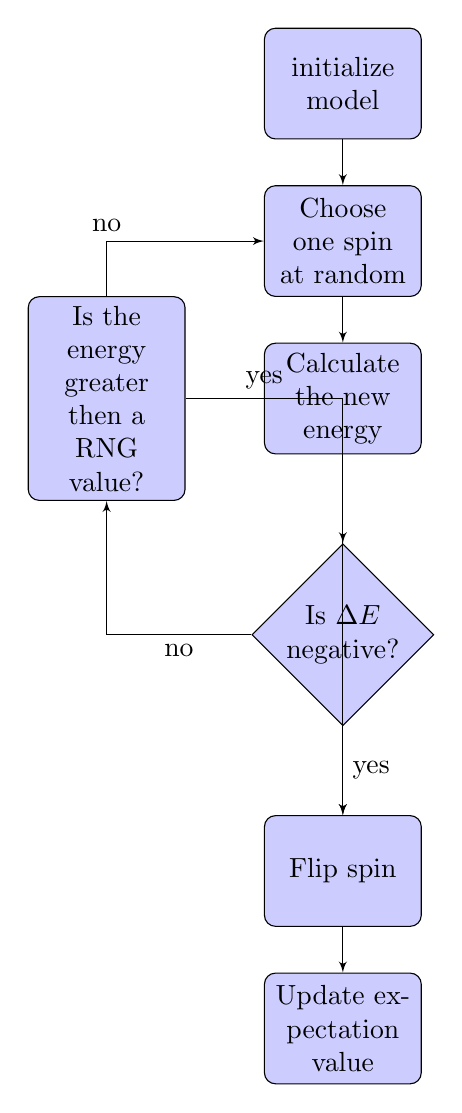
\begin{tikzpicture}[node distance = 2cm, auto]
% Place nodes
\node [block] (init) {initialize model};
\node [block, below of=init] (identify) {Choose one spin at random};
\node [block, below of=identify] (evaluate) {Calculate the new energy};
\node [block, left of=evaluate, node distance=3cm] (update) {Is the energy greater then a RNG value?};
\node [decision, below of=evaluate] (decide) {Is $\Delta E$ negative?};
\node [block, below of=decide, node distance=3cm] (stop) {Flip spin};
\node [block, below of=stop, node distance=2cm] (finnished) {Update expectation value};
% Draw edges
\path [line] (init) -- (identify);
\path [line] (identify) -- (evaluate);
\path [line] (evaluate) -- (decide);
\path [line] (decide) -| node [near start] {no} (update);
\path [line] (update) -| node [near start] {yes} (stop);
\path [line] (update) |- node {no} (identify);
\path [line] (decide) -- node {yes}(stop);
\path [line] (stop) -- (finnished);
\end{tikzpicture}
\end{comment}




\subsection{Tricks}

The strategy outlined above requires one to calculate a change in energy. This as it turns out is computationally expensive to calculate exponentials. Fortunately it is possible to circumvent this. For a two dimensional lattice it is possible to precalculate all the energy states, so when prompted to calculate the exponential it is possible to just insert the precalculated exponential. This saves some time and computing power. The change in energy and magnetic moment can be shown to be in the form \cite{compphys}:

\begin{align*}
	\Delta E=&2Js_{\text{before}}\sum_{\langle k\rangle}s_k&\Delta M=-2Js_{\text{before}}
\end{align*}

Here the sum is over the surrounding spins $j$, and the $s_{\text{before}}$ is the spin before the flip.

























%implementation
\section{Implementation}

The Metropolis algorithm was implemented in the program called main\_\_\_.cpp where the underscores gives different versions of the program main.cpp. The different versions has different ways to write to file.


The structure of the Metropolis algorithm makes is possible to parallelize some of the tasks. The parallelization utilizes the structure of the metropolis algorithm though it being possible to work in many parts at the same time. The overall tasks will still be the same so a great del of the code in the parallelized and non parallelized versions will be the same. The parallelization saves some time for the user, but requires more threads to do. Each thread has a unique number(rank), this makes it possible to use this tag to give out the temperature each thread is working with. I have chosen to implement MPI.













%result
\section{Results}



\subsection{Parallelization}
 
The parallelized version should be almost a factor of $\text{threads}-1$ times faster. The reason why it is not exact, or close to exact, is because each thread has to be initialized, terminated and exchange data. This takes some time taking away some of the speed. This was tested in a lab-session but the results are not included in the table below. These factors becomes less and less important with increasing lattice sizes. Another important factor was the chipset of the computer. The initial trial ran on a stationary computer with a E$4800$ intel chip. This does not have hyperthreading and will therefore have a more linear scale. The table below was made using a macbook pro with a chip that does have hyperthreading.\footnote{\href{https://www.intel.com/content/www/us/en/architecture-and-technology/hyper-threading/hyper-threading-technology.html}{Intel Hyper-Threading}}. 
This actually makes the difference between the parallelized and non parallelized version bigger than expected. 
 
 
\begin{center}
 	\label{tab:parallell}
 	\captionof{table}{The grids ran for 50'000 Monte Carlo cycles. Expected difference for a nonhyperthreaded CPU is given in the fourth collomn.}
 	\begin{tabularx}{\textwidth}{c X c X c X c X c}
 		\hline 
 		Latttice size && One thread && parallel && Exp. dif. && Actual difference\\ 
 		\hline
 		40x40   	&&      15.251s	&&		5.991 s 	&&	2.000	&&	2.546	\\  
 		60x60   	&&      33.923s	&&		13.351 s	&&	2.000	&&	2.541	\\
 		100x100   	&&      92.584s	&&		36.245 s	&&	2.000	&&	2.554	\\
 		\hline
 	\end{tabularx}
\end{center}
 
 
\begin{center}
 	\label{tab:expected-time}
 	\captionof{table}{The table shows the exprected time development vs the actual time development. }
 	\begin{tabularx}{\textwidth}{c X c X c X c}
 		\hline 
 		Size && Expected time && Actual time && $\frac{T_{i}}{T_{40}}$\\ 
 		\hline
 		40x40   	&&      x		&&		8.490 s 	&&	1.000	\\  
 		60x60   	&&      2.25x	&&		19.350 s	&&	2.279	\\
 		100x100   	&&      6.25x	&&		54.068 s	&&	6.368	\\
 		\hline
 	\end{tabularx}
\end{center}
 


\subsection{2x2 lattice}


\subsubsection{Analytical result}

The possible states for a $2\cross 2$ lattice can be quite easily be found due to the small size off the lattice. From this the analytical partition function can be found. To find the partition function one has to find all the possible microstates of the system, and from them calculate the energies. Note that the boundary condition outlined in the theory section is used.

\begin{center}
\label{tab:states-2x2}
\captionof{table}{The table shows all the different microstates possible for the system. A third collomn also shows the magnetic moment of these states. The left and right hand side states shows the mirroring effect caused by a flip of all spins creating the state.}
\begin{tabularx}{\textwidth}{|c c c |X| c c c|}
    \hline
    \hline 
        State & Energy & Magnetic moment && State & Energy & Magnetic moment \\ 
    \hline
    \hline
        \tilstand{1}{1}{1}{1} & -8J & 4 && \tilstand{0}{0}{0}{0} & -8J & -4 \\
        \hline
        \tilstand{0}{1}{1}{1} & 0J & 2 && \tilstand{1}{0}{0}{0} & 0J & -2 \\ 
        \hline
        \tilstand{1}{0}{1}{1} & 0J & 2 && \tilstand{0}{1}{0}{0} & 0J & -2 \\ 
        \hline
        \tilstand{1}{1}{0}{1} & 0J & 2 && \tilstand{0}{0}{1}{0} & 0J & -2 \\ 
        \hline
        \tilstand{1}{1}{1}{0} & 0J & 2 && \tilstand{0}{0}{0}{1} & 0J & -2 \\
        \hline
        \tilstand{0}{0}{1}{1} & 0J & 0 && \tilstand{1}{1}{0}{0} & 0J & 0 \\ 
        \hline
        \tilstand{0}{1}{0}{1} & 0J & 0 && \tilstand{1}{0}{1}{0} & 0J & 0 \\ 
        \hline
        \tilstand{1}{0}{0}{1} & 8J & 0 && \tilstand{0}{1}{1}{0} & 8J & 0 \\ 
    \hline
    \hline
\end{tabularx}
\end{center}



\begin{center}
\label{tab:states-2x2-summary}
\captionof{table}{Summary of all the states given in the table above. }
\begin{tabularx}{\textwidth}{|c| X c| X c| X c|}
    \hline 
    \hline 
        Number of $\color{black}{\uparrow}$ && Multiplicity && Energy && Magnetic moment \\ 
    \hline
        4   &&      1      &&      -8J     &&       4       \\  
        3   &&      4      &&      0J      &&       2       \\
        2   &&      2      &&      8J      &&       0       \\
        2   &&      4      &&      0J      &&       0       \\
        1   &&      4      &&      0J      &&       -2      \\
        0   &&      1      &&      -8J     &&       -4      \\
    \hline
\end{tabularx}
\end{center}


The analytical value for the partition function $Z$ is now found by summing over all these states:

\begin{align*}
    &Z = \sum_{\text{microstates}=i} e^{-\beta E_i}\\
    &Z = \sum_{\text{microstates}=i}e^{-\beta E_i}=2e^{8}+2e^{-8}+12
\end{align*}

Summing over the product of the energy value and the probability of that energy state gives the expectation value:


\begin{align*}
    &\langle E \rangle = \sum_{\text{microstates}=i} E_iP(E_i)\\
    &=\frac{1}{Z} \sum_{\text{microstates}=i} E_i e^{-E_i}\\
    &=\frac{1}{Z} \left( -16 e^8 + 16e^{-8} \right) = -7.984\\ 
    &\frac{\langle E \rangle }{N}= \frac{\langle E \rangle}{4} = -1.996
\end{align*}


The same procedure is used to sum over all the magnetic states to find the mean magnetic moment:

\begin{align*}
    &\langle |M| \rangle = \sum_{\text{microstates}=i} M_iP(E_i)\\
    &= \frac{1}{Z} \sum_i M_i e^{-E_i}\\
    &= \frac{1}{Z}\left(4\cdot1e^{8}+2\cdot4e^{0}+ 0\cdot2e^{-8}+0\cdot4e^{0}+2\cdot4e^{0}+4\cdot1e^{8}\right)\\
    &=\frac{1}{Z}\left(16+8e^{8}\right) = 3.995\\
    &\frac{\langle |M| \rangle }{N}= \frac{\langle |M| \rangle}{4} = 0.999
\end{align*}


The heat capacity $C_v$ is the change in energy per temperature and can be found by taking the derivative of the expectation value of the energy. Another way of finding the heat capacity is by $\langle E^2 \rangle - \langle E \rangle^2$:

\begin{align*}
    &\langle E^2 \rangle = \sum_{\text{microstates}=i} E_i^2P(E_i)\\
    &=\frac{1}{Z} \sum_{\text{microstates}=i} E_i^2 e^{-E_i}\\
    &=\frac{1}{Z} \left( 128 e^8 + 128 e^{-8} \right)\\
    &C_V = \langle E^2 \rangle - \langle E \rangle^2 = 0.12832\\ 
    &\frac{C_V}{N}= 0.0321
\end{align*}


The magnetic suseptibility is found the same way, but for the magnetic moment:

\begin{align*}
    &\langle M^2 \rangle = \sum_{\text{microstates}=i}M_i^2P(E_i)\\
    &= \frac{1}{Z} \sum_{\text{microstates}=i} M_i^2 e^{-E_i}\\
    &= \frac{1}{Z} \left(16\cdot1e^{8}+4\cdot4e^{0}+0\cdot2e^{-8}+
    0\cdot4e^{0}+4\cdot4e^{0}+16\cdot1e^{8}\right)\\
    &=\frac{1}{Z}\left(32+32e^{8}\right)=15.973\\
    &\langle \chi \rangle=\langle M^2 \rangle - \langle M \rangle^2 = 0.0160\\
    &\frac{\langle \chi \rangle}{N} = 0.00401
\end{align*}



\subsubsection{Numerical results}

For the results that follows the program was ran with $10^5$ Monte Carlo cycles. First all the results are shown, then a error estimate with a converges evaluation is given.




\begin{figure}[H]
    \centering
    \begin{subfigure}{0.5\textwidth}
        \centering
        \includegraphics[width=\linewidth]{result/bilder/2x2/energy22}
        \caption{}
    \end{subfigure}%
    ~ 
    \begin{subfigure}{0.5\textwidth}
    	\centering
    	\includegraphics[width=\linewidth]{result/bilder/2x2/cv22_}
    	\caption{}
    \end{subfigure}
    \begin{subfigure}{0.5\textwidth}
        \centering
        \includegraphics[width=\linewidth]{result/bilder/2x2/mabs22}
        \caption{}
    \end{subfigure}%
    ~ 
    \begin{subfigure}{0.5\textwidth}
        \centering
        \includegraphics[width=\linewidth]{result/bilder/2x2/chi22}
        \caption{}
    \end{subfigure}
    \caption{a) Subplots shows how the expectation value for the different values varies, plotted with the number of Monte Carlo cycles on the x-axis.}
    \label{22results}
\end{figure}


As one can see from the graphs above the values tends quicly towards the numerically found expectation value. Below is a plot showing the difference between the numerical and analytical solutions. This will just be a rescaling of the plots. From these plots it is a good approximation when the Monte Carlo simulation has done about $40\%$ of the cycles. At this point there is almost no difference between the numerical and analytical solutions.


\begin{figure}[H]
	\centering
	\begin{subfigure}{0.5\textwidth}
		\centering
		\includegraphics[width=\linewidth]{result/bilder/2x2/energyerror22}
		\caption{}
	\end{subfigure}%
	~ 
	\begin{subfigure}{0.5\textwidth}
		\centering
		\includegraphics[width=\linewidth]{result/bilder/2x2/cverror22_}
		\caption{}
	\end{subfigure}
	\begin{subfigure}{0.5\textwidth}
		\centering
		\includegraphics[width=\linewidth]{result/bilder/2x2/mabserror22}
		\caption{}
	\end{subfigure}%
	~ 
	\begin{subfigure}{0.5\textwidth}
		\centering
		\includegraphics[width=\linewidth]{result/bilder/2x2/chierror22}
		\caption{}
	\end{subfigure}
	\caption{a) Shows how the the error develops for all the different expectation values.}
	\label{22error}
\end{figure}








\subsection{Numerical 20x20}

At this point no analytical solution is found, so from here on only the numerical solution is studied. All plots were made with $10*10^6$ cycles. For the $20\times20$ grid who different starting points where analyzed. On the right side a plot with random spin configuration in initialized. While on the left hand side the system is initialized with all spins in the same direction. Firstly the energy and magnetic moment is analyzed for $T=1$. Then a higher temperature state is analyzed with $T=2.4$

\begin{figure}[H]
    \centering
    \begin{subfigure}{0.5\textwidth}
        \centering
        \includegraphics[width=\linewidth]{result/bilder/20x20/E-N20-T1}
        \caption{}
    \end{subfigure}%
    ~ 
    \begin{subfigure}{0.5\textwidth}
        \centering
        \includegraphics[width=\linewidth]{result/bilder/20x20/E-N20-T1-RNG}
        \caption{}
    \end{subfigure}
    \caption{The figure shows the development of the energy. In the program $T$ is sat to $1$. }
    \label{fig:}
\end{figure}

\begin{figure}[H]
    \centering
    \begin{subfigure}{0.5\textwidth}
        \centering
        \includegraphics[width=\linewidth]{result/bilder/20x20/M-N20-T1}
        \caption{}
    \end{subfigure}%
    ~ 
    \begin{subfigure}{0.5\textwidth}
        \centering
        \includegraphics[width=\linewidth]{result/bilder/20x20/M-N20-T1-RNG}
        \caption{}
    \end{subfigure}
    \caption{The figure shows the development of the Magnetic moment. In the program $T$ is sat to $1$. }
    \label{fig:}
\end{figure}

A clear trend is visible for the initialized ordered case. This has more irregularities and uses longer time to reach equilibrium. This is because it started out ordered in a manner that was not energetically beneficial for the system. Whereas the random initialized case has a much smoother curve due to it starting in a more energetically favored position. For the next plots the temperature was increased, to look at the effects temperature has on the system.




\begin{figure}[H]
    \centering
    \begin{subfigure}{0.5\textwidth}
        \centering
        \includegraphics[width=\linewidth]{result/bilder/20x20/E-N20-T24}
        \caption{}
    \end{subfigure}%
    ~ 
    \begin{subfigure}{0.5\textwidth}
        \centering
        \includegraphics[width=\linewidth]{result/bilder/20x20/E-N20-T24-RNG}
        \caption{}
    \end{subfigure}
    \caption{The figure shows the development of the energy. In the program $T$ is sat to $2.4$.}
    \label{fig:}
\end{figure}

\begin{figure}[H]
    \centering
    \begin{subfigure}{0.5\textwidth}
        \centering
        \includegraphics[width=\linewidth]{result/bilder/20x20/M-N20-T24}
        \caption{}
    \end{subfigure}%
    ~ 
    \begin{subfigure}{0.5\textwidth}
        \centering
        \includegraphics[width=\linewidth]{result/bilder/20x20/M-N20-T24-RNG}
        \caption{}
    \end{subfigure}
    \caption{The figure shows the development of the Magnetic moment. In the program $T$ is sat to $2.4$.}
    \label{fig:}
\end{figure}

For the higher temperature the Helmholtz free energy equations temperature term becomes more impactull. $F=E-TS$. This is visible in the random initialized version. This is now not so smooth and varies more. In all of these cases, for $T=1$ and $T=2.4$ the same variations in the first part of the cycles can be observed. The next plot hows what the plots for $T=1$ would have looked like if the first $10^5$ steps are not included.


\begin{figure}[H]
    \centering
    \begin{subfigure}{0.5\textwidth}
        \centering
        \includegraphics[width=\linewidth]{result/bilder/20x20/E-N20-T1-Term}
        \caption{}
    \end{subfigure}%
    ~ 
    \begin{subfigure}{0.5\textwidth}
        \centering
        \includegraphics[width=\linewidth]{result/bilder/20x20/M-N20-T1-Term}
        \caption{}
    \end{subfigure}
    \caption{The development of energy when $T = 1$, excluding the first $10^5$ steps.  }
    \label{fig:equilibrium}
\end{figure}


For the remainder of the report $10^5$ Monte Carlo cycles will be used to obtain equilibrium. This is a value chosen because if more cycles were chosen this would require more computing power, if less cycles were chosen then the results would not give the approximate expectation value. 












\subsection{Accepted configurations}

In the previous section the differences between temperature and initial states were studied. In this section a study of the acceptance rate of flips is made, not focusing on the energy or magnetic moment of the system. As for the previous section, left figures shows a ordered initial configuration while the right hand side shows a random starting point.

\begin{figure}[H]
    \centering
    \begin{subfigure}{0.5\textwidth}
        \centering
        \includegraphics[width=\linewidth]{result/bilder/config/energy22-MC1000000T1-configN20}
        \caption{}
    \end{subfigure}%
    ~ 
    \begin{subfigure}{0.5\textwidth}
        \centering
        \includegraphics[width=\linewidth]{result/bilder/config/energy22-MC1000000T1-config-RNGN20}
        \caption{}
    \end{subfigure}
    \caption{Plot shows the acceptance rate of flipped spins at temperature one, with $10^6$ cycles. }
    \label{fig:config-T1}
\end{figure}
The right configuration seems to have a lower acceptance rate then the left one. This is due to the scaling and first steps. When looking at the y-axis one can see that for the right configuration acceptance is high. 

\begin{figure}[H]
    \centering
    \begin{subfigure}{0.5\textwidth}
        \centering
        \includegraphics[width=\linewidth]{result/bilder/config/energy22-MC1000000T24-configN20}
        \caption{}
    \end{subfigure}%
    ~ 
    \begin{subfigure}{0.5\textwidth}
        \centering
        \includegraphics[width=\linewidth]{result/bilder/config/energy22-MC1000000T24-config-RNGN20}
        \caption{}
    \end{subfigure}
    \caption{Plot shows the acceptance rate of flipped spins at temperature $2.4$, with $10^6$ cycles. }
    \label{fig:config-T24}
\end{figure}

When comparing the two different temperatures the change in acceptance rate is noticeable. For higher temperatures the acceptance rate becomes over a factor of ten larger. 


\subsection{Probability distribution}

The probability distribution of energies for the two different temperatures are extreme.

\begin{figure}[H]
    \centering
    \begin{subfigure}{0.5\textwidth}
        \centering
        \includegraphics[width=\linewidth]{result/bilder/hist/MC1000000T1-distN20-hist}
        \caption{}
    \end{subfigure}%
    ~ 
    \begin{subfigure}{0.5\textwidth}
        \centering
        \includegraphics[width=\linewidth]{result/bilder/hist/MC1000000T24-distN20-hist}
        \caption{}
    \end{subfigure}
    \caption{The two figures shows the distribution of energy states at different temperatures. The left plot shows the distribution at temperature $1$ and the right plot shows the distribution at temperature $2.4$.}
    \label{fig:tc-chi-cv}
\end{figure}

The differences in distribution is due to the Boltzmann distribution used in the model. For the lowest temperature more states are expected to have the lower energy, while for the system with higher energy the distribution is expected to have a better distribution of energies. This also fits the results from the previous section well. For higher temperatures the system accepts more changes and the peak becomes broader. While for the low temperature few changes were accepted leading to a lower degree peak broadening.




















\subsection{Phase transition}

To study the phase transitions of the system several runs were done varying $L$ between $20-200$. The figures below shows a selection of the runs.


\begin{figure}[H]
    \centering
    \begin{subfigure}{0.5\textwidth}
        \centering
        \includegraphics[width=\linewidth]{result/bilder/Tc/e-Tc}
        \caption{}
    \end{subfigure}%
    ~ 
    \begin{subfigure}{0.5\textwidth}
        \centering
        \includegraphics[width=\linewidth]{result/bilder/Tc/m-Tc}
        \caption{}
    \end{subfigure}
    \begin{subfigure}{0.5\textwidth}
    	\centering
    	\includegraphics[width=\linewidth]{result/bilder/Tc/chi-Tc}
    	\caption{}
    \end{subfigure}%
    ~ 
    \begin{subfigure}{0.5\textwidth}
    	\centering
    	\includegraphics[width=\linewidth]{result/bilder/Tc/cv-Tc}
    	\caption{}
    \end{subfigure}
    \caption{Figures show the results for different temperatures $T$ plottet against energy(a), magnetisation(b), magnetic susceptibility(c) and heat capacity(d)}
    \label{fig:tc-chi-cv}
\end{figure}

The trends for the heat capacity shows a peak position. This should in theory correspond to the critical temperature. From the data it is clear that more data points are required to get a better result. Comparing the critical temperature to the magnetization gives a dip in magnetization close to the critical temperature. If the plots had been extended more two visible magnetization linear trends should be visible. One on each side of the phase transition. 










\pagebreak
\subsubsection{Critical temperature}
In the theory section a formula for the critical temperature was given. 

\begin{align*}
     &T_C (L) - T_C (L=\infty) = a L^{\frac{-1}{v}}
\end{align*}

 \begin{align*}
     &T_C (L_i) - T_C (L_j) = a 
     \left(
     L_i^{\frac{-1}{v}}-L_j^{\frac{-1}{v}}
     \right)
     \\
     &a = 
     \frac{T_C (L_i) - T_C (L_j)} 
     {
     L_i^{\frac{-1}{v}}-L_j^{\frac{-1}{v}}
     }
 \end{align*}
Applying this formula to the $L_i$ and $L_j$ plotted above gives a change in the variable $a$. The phase transistions are taken from the plots above. The cange in the variable $a$ will also be affected by ones choise of critical temperature. In this case the critical temperatures would be better if one had included more data points in the plot.

\begin{center}
\label{tab:extracting a}
\captionof{table}{The table shows how a differ for different $L_i$ and $L_j$  one uses.}
\begin{tabularx}{\textwidth}{|c| X c| X c| X c| X l|}
    \hline 
        $L_i$ && $L_j$ && $T_{C_i}$ && $T_{C_j}$ && a\\ 
    \hline
        60      &&      100     &&  2.30  &&  2.29  && 0.00025 \\
        60      &&      140     &&  2.30  &&  2.28  && 0.00025 \\
        60      &&      200     &&  2.30  &&  2.27  && 0.0002142 \\
        100     &&      140     &&  2.29  &&  2.28  && 0.00025 \\
        100     &&      200     &&  2.29  &&  2.27  && 0.0002 \\
        140     &&      200     &&  2.28  &&  2.27  && 0.0001666 \\
    \hline
\end{tabularx}
\end{center}

To get a common $T_C(\infty)$ the average of the different $a$'s are found. This is then plugged into the formula for $T_C(\infty)$. The results of $T_C(\infty)$ with the average $a$ is given in the table below:

\begin{center}
\label{tab:t-c}
\captionof{table}{Table giving $T_C(\infty)$ when the average of the variable $a$ is used.}
\begin{tabularx}{\textwidth}{|c| X c| X c| X |c| }
    \hline 
        $L_i$ && $T_C(L_i)$ && $T_C(\infty)$ \\ 
    \hline
        60      &&  2.30  && 2.2999\\
        100     &&  2.29  && 2.2899\\
        140     &&  2.28  && 2.2799\\
        200     &&  2.27  && 2.2699\\
    \hline
\end{tabularx}
\end{center}

An alternative way of finding $T_C$ is possible by linear regression of a plot with the different finite $T_C$ values plotted against the inverse of $L$. The intersection point of this regression line with the y-axis would give $T_C$ for a infinite lattice.










%conclusion
\section{Conclusion}



Ihe Ising model has in this project been used to study some of the basic physical properties of a two dimensional lattice. A two dimensional model was analyzed both analytically and numerical and the results were compared. The numerical approach gave accurate results within what can be expected for a numerical model. For this system $10^5$ cycles was necessary to reach convergence. The system was then expanded to a $20\times20$ lattice. Here only the numerical approach was possible due to the challenges faced with the partition function in the analytical approach. The system was then sat to two different temperatures and further studies on the steady state and acceptance frequency was made. Here temperature was found to increase the jump frequency, and broaden the range of energy states in the system.
Lastly a phase transition of the system was analyzed and a critical temperature was found. The critical temperature was close to the temperature found by Onsager.

The largest room for improvement found be to increase the amount of points used in the phase transition calculations. This plot, at least visually looked like it had room for improvement with more datapoints. The reason why this was not done in this project was due to limited computational power.
































\printbibliography


\end{document}